%% LyX 2.3.6.1 created this file.  For more info, see http://www.lyx.org/.
%% Do not edit unless you really know what you are doing.
\documentclass[english]{article}
\usepackage[T1]{fontenc}
\usepackage[latin9]{inputenc}
\usepackage{geometry}
\geometry{verbose,tmargin=2.5cm,bmargin=2.5cm,lmargin=2.5cm,rmargin=2.5cm}
\usepackage{calc}
\usepackage{textcomp}
\usepackage{graphicx}
\PassOptionsToPackage{normalem}{ulem}
\usepackage{ulem}

\makeatletter

%%%%%%%%%%%%%%%%%%%%%%%%%%%%%% LyX specific LaTeX commands.
%% Because html converters don't know tabularnewline
\providecommand{\tabularnewline}{\\}

\makeatother

\usepackage{babel}
\begin{document}
{[}SPLIT\_HERE{]}
\begin{enumerate}
\item \textbf{{[}DHS/PRELIM/9569/2021/P1/Q1{]} }

A cosmic ray striking computer memory at just the right time can flip
a bit, turning a 0 into a 1 or vice versa. 

Bit flips had caused plane accidents, software glitches, and at times,
the Blue Screen of Death (BSoD) on personal computers. 
\begin{enumerate}
\item The hexadecimal number \texttt{D4} had been changed to \texttt{9A}.
Suggest the minimum number of times a bit flip could have affected
it and explain why. \hfill{}{[}2{]}
\item Explain why Unicode characters, as compared to ASCII characters, are
more likely to be altered after a cosmic ray strike.\hfill{} {[}2{]}
\item Define what a backup and archive is, and explain which should be prioritised
if a company is warned of a global cosmic ray strike occurring in
a week. \hfill{}{[}4{]}
\item Explain how TCP/IP layers help to fulfil the purpose of the TCP/IP
model. \hfill{}{[}2{]}
\item Suggest and explain a consequence on network communication when a
data packet is affected by a bit flip occurring at the Internet Layer\hfill{}
{[}2{]}
\item Explain why the consequence of a bit flip occurring at the Internet
Layer and the Transport Layer would be the same as the consequence
as a bit flip occurring at the Internet Layer only. \hfill{}{[}1{]}
\end{enumerate}
{[}SPLIT\_HERE{]}
\item \textbf{{[}DHS/PRELIM/9569/2021/P1/Q2{]} }

An array stores 16 powers of 2 integers in ascending order: 

1, 2, 4, 8, 16, 32, 64, 128, 256, 512, 1024, 2048, 4096, 8192, 16384,
32768 
\begin{enumerate}
\item If the array is searched by means of a binary search, state which
elements would be accessed, and in what order,
\begin{enumerate}
\item when searching for the number 4096 (which is present), and \hfill{}{[}1{]}
\item when searching for the number 3 (which is not present). \hfill{}{[}1{]}
\end{enumerate}
\item Draw a program flowchart of an iterative binary search algorithm.
\hfill{}{[}6{]}
\item Explain why binary search could be more efficient than linear search.
\hfill{} {[}1{]}
\item State the time complexities of hash table search and binary search
and explain which is more efficient with reference to their time complexities
in the above scenario. \hfill{} {[}4{]}
\end{enumerate}
{[}SPLIT\_HERE{]}
\item \textbf{{[}DHS/PRELIM/9569/2021/P1/Q3{]} }

A mobile network provider\textquoteright s management of customer\textquoteright s
overdue bills include an automated emailing and SMS system. 
\begin{itemize}
\item If a mobile bill is overdue, a daily system generated reminder is
emailed to the user indicating the overdue details. 
\item If the user has 1 mobile bill that is more than 6 days overdue, in
place of the daily reminder email, a warning email and SMS will be
sent to the user. 
\item If a user has more than 4 bills which are more than 14 days overdue,
the user will incur a penalty fee for every additional week starting
from the 14th day of being overdue.
\item If a user has incurred more than 3 penalty fees, the user\textquoteright s
mobile service will be terminated. 
\item Penalty fees could be incurred as a result of other actions such as
accessing illegal websites. 
\item Each bill issued to a customer represents the past month\textquoteright s
usage. 
\end{itemize}
\begin{enumerate}
\item Create a decision table showing all possible outcomes and results
for bill(s) that are overdue. \hfill{}{[}4{]}
\item Simplify the decision table by removing redundancies. \hfill{}{[}3{]}
\item A user interface is designed for a program for customers to check
their bills and overdue status. State a usability principle and describe
how the user interface of the program should be designed to demonstrate
this principle.\hfill{} {[}2{]}
\end{enumerate}
{[}SPLIT\_HERE{]}
\item \textbf{{[}DHS/PRELIM/9569/2021/P1/Q4{]} }
\begin{enumerate}
\item Explain how a linked list data structure could be more suitable than
an array data structure to implement a binary tree. \hfill{}{[}2{]}
\item (b) Suggest and justify one circumstance where an array structure
is more appropriate than a linked structure. \hfill{}{[}2{]}
\end{enumerate}
The diagram shows a binary tree before and after an inversion. 
\begin{center}
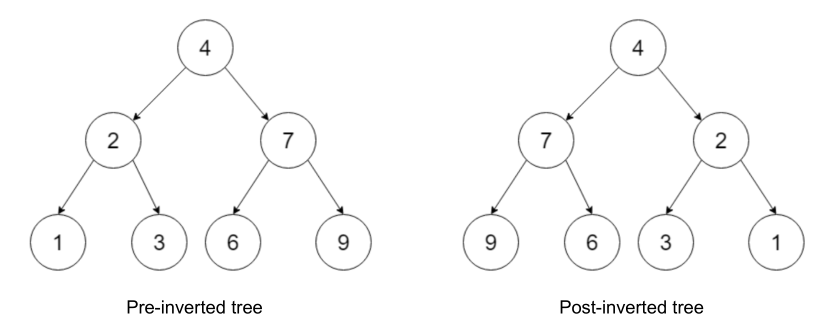
\includegraphics[width=0.5\paperwidth]{C:/Users/Admin/Desktop/Github/question_bank/static/img/9597-DHS-2021-P1-Q4-1}
\par\end{center}

Each node has these attributes: 
\begin{itemize}
\item \texttt{right} which is the pointer to right subtree 
\item \texttt{data} which is the value contained in each respective node
displayed above 
\item \texttt{left} which is the pointer to the left subtree
\end{itemize}
\begin{enumerate}
\item[(c)]  Write pseudocode for procedure \texttt{insert} which will add a
node to the post-inverted tree (which may be empty) in such a way
that if the new value of the node is \textbf{less} than the value
at the current node, the new node will be added to the \textbf{right}
subtree, or else it will be added to the left subtree. \texttt{insert}
takes in values \texttt{node\_data} and \texttt{root\_node} which
is the value to be added to the tree and the instance of the root
node of the tree respectively. \hfill{}{[}6{]}
\item[(d) ] A function \texttt{invertTree} takes in the root node of the above
pre-inverted tree, uses recursion to invert it into the post-inverted
tree, and returns the root node of the post-inverted tree. Write pseudocode
for the function and visualise it in a trace diagram. An incomplete
trace diagram is provided for you to begin with. Copy and complete
it. 
\noindent \begin{center}
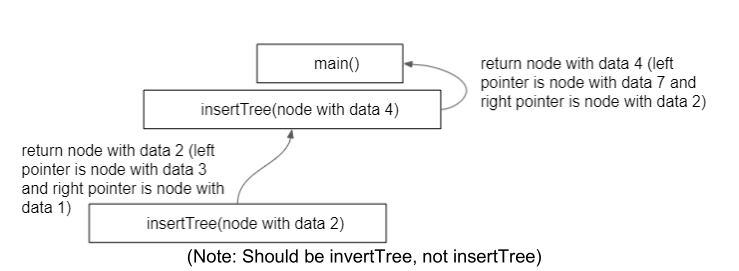
\includegraphics[width=0.5\paperwidth]{C:/Users/Admin/Desktop/Github/question_bank/static/img/9597-DHS-2021-P1-Q4-2}
\par\end{center}

(Note: Should be invertTree, not insertTree) \hfill{}{[}6{]}
\end{enumerate}
{[}SPLIT\_HERE{]}
\item \textbf{{[}DHS/PRELIM/9569/2021/P1/Q5{]} }

Consider the following data which shows a single Civics Group record
used in COVID19 vaccination tracking. 
\noindent \begin{center}
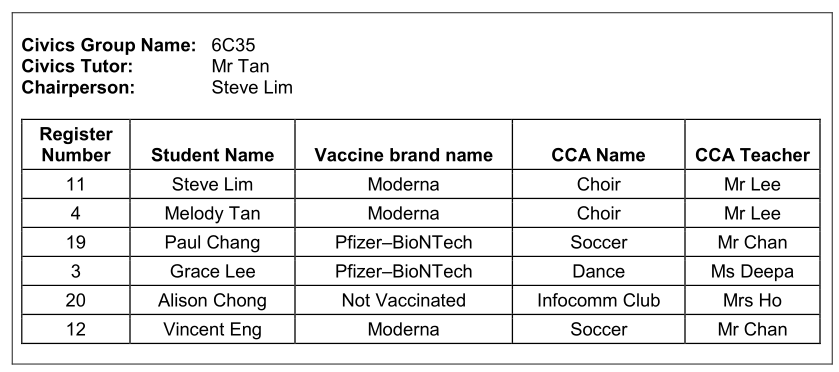
\includegraphics[width=0.5\paperwidth]{C:/Users/Admin/Desktop/Github/question_bank/static/img/9597-DHS-2021-P1-Q5}
\par\end{center}
\begin{enumerate}
\item Derive a set of tables to show the above data in first, second and
third normal form. \hfill{}{[}6{]}
\item Draw an ER diagram for a normalised database design. \hfill{} {[}2{]}
\item Using examples in the above context, explain the significance of the
following terms:
\begin{enumerate}
\item primary key \hfill{}{[}2{]}
\item foreign key \hfill{}{[}2{]}
\end{enumerate}
\item With reference to the above context, describe or suggest a scenario
where a NoSQL database would be more appropriate. \hfill{} {[}1{]}
\end{enumerate}
{[}SPLIT\_HERE{]}
\item \textbf{{[}DHS/PRELIM/9569/2021/P1/Q6{]} }

Long-distance optical fibre lines and submarine cables which are a
vital part of the global internet infrastructure are vulnerable to
solar superstorms which happen once in a century. The last solar superstrom
was in 1921. 
\begin{enumerate}
\item State and explain why websites would or would not be accessible by
web browsers if a solar superstorm shuts down all DNS servers. \hfill{}{[}2{]}
\item Explain packet switching and its importance in ensuring global internet
connectivity when some parts of the earth are hit by a solar superstorm.
\hfill{}{[}4{]}
\end{enumerate}
An international company based in many countries updates its network
structure to ensure Internet connectivity during solar superstorms. 

Employees can now access files on a shared virtual space which is
made up of 3 servers located in the United States, Europe, and Asia.
All servers hold identical information (any changes made on one server
would update the other servers immediately) so even if one server
is affected by the solar superstorm, employees still can access their
files on the other servers. 

Employees must be connected physically to the company\textquoteright s
intranet network at each country\textquoteright s office to access
the virtual space. 
\begin{enumerate}
\item[(c)] Draw a network diagram of the above configuration and label the LAN,
internet, router(s), WAN link(s), intranet, servers, and employee
laptops. \hfill{}{[}5{]}
\item[(d)] Why is version control vital when employees from different countries
work in teams? \hfill{}{[}1{]}
\end{enumerate}
{[}SPLIT\_HERE{]}
\item \textbf{{[}DHS/PRELIM/9569/2021/P1/Q7{]} }

A divide and conquer approach is used by merge sort to successively
divide a list into half, forming two sublists, until each sublist
is of length 1. The sublists are then sorted and merged into larger
sublists until they are recombined into a single sorted list. An algorithm
for merge sort to perform an ascending sort is given below. It will
be used to sort large or small data sizes. 

\noindent %
\noindent\begin{minipage}[t]{1\columnwidth}%
\texttt{01 PROCEDURE mergesort(mergelist : ARRAY) }

\texttt{02}

\texttt{03 \qquad{}IF LENGTH(mergelist) > 1 THEN }

\texttt{04 }

\texttt{05 \qquad{}\qquad{}mid \textleftarrow{} LENGTH(mergelist)
DIV 2 }

\texttt{06 }

\texttt{07 \qquad{}\qquad{}FOR index \textleftarrow{} 0 TO (mid
- 1) }

\texttt{08 \qquad{}\qquad{}\qquad{}lefthalf{[}index{]} \textleftarrow{}
mergelist{[}index{]} }

\texttt{09 \qquad{}\qquad{}NEXT index}

\texttt{10}

\texttt{11 \qquad{}\qquad{}right\_len \textleftarrow{} LENGTH(mergelist)
- mid}

\texttt{12}

\texttt{13 \qquad{}\qquad{}FOR index \textleftarrow{} 0 TO (right\_len
- 1) }

\texttt{14 \qquad{}\qquad{}\qquad{}righthalf{[}index{]} \textleftarrow{}
mergelist{[}right\_len + index{]} }

\texttt{15 \qquad{}\qquad{}NEXT index }

\texttt{16}

\texttt{17 \qquad{}\qquad{}mergesort(lefthalf) }

\texttt{18 \qquad{}\qquad{}mergesort(righthalf) }

\texttt{19}

\texttt{20 \qquad{}\qquad{}i \textleftarrow{} 0 }

\texttt{21 \qquad{}\qquad{}j \textleftarrow{} 0 }

\texttt{22 \qquad{}\qquad{}k \textleftarrow{} 0 }

\texttt{23 \qquad{}\qquad{}WHILE i < LENGTH(lefthalf) AND j < LENGTH(righthalf) }

\texttt{24 \qquad{}\qquad{}\qquad{}IF lefthalf{[}i{]} > righthalf{[}j{]}
THEN }

\texttt{25 \qquad{}\qquad{}\qquad{}\qquad{}mergelist{[}k{]} \textleftarrow{}
lefthalf{[}i{]}}

\texttt{26 \qquad{}\qquad{}\qquad{}\qquad{}i \textleftarrow{}
i + 1 }

\texttt{27 \qquad{}\qquad{}\qquad{}ELSE }

\texttt{28 \qquad{}\qquad{}\qquad{}\qquad{}mergelist{[}k{]} \textleftarrow{}
righthalf{[}j{]} }

\texttt{29 \qquad{}\qquad{}\qquad{}\qquad{}j \textleftarrow{}
j + 1 }

\texttt{30 \qquad{}\qquad{}\qquad{}ENDIF }

\texttt{31 \qquad{}\qquad{}\qquad{}k \textleftarrow{} k + 1}

\texttt{32 \qquad{}\qquad{}ENDWHILE }

\texttt{33}

\texttt{34 \qquad{}\qquad{}WHILE i < LENGTH(lefthalf) }

\texttt{35 \qquad{}\qquad{}\qquad{}mergelist{[}k{]} \textleftarrow{}
lefthalf{[}i{]} }

\texttt{36 \qquad{}\qquad{}\qquad{}i \textleftarrow{} i + 1 }

\texttt{37 \qquad{}\qquad{}\qquad{}k \textleftarrow{} k + 1 }

\texttt{38 \qquad{}\qquad{}ENDWHILE }

\texttt{39}

\texttt{40 \qquad{}\qquad{}WHILE j < LENGTH(righthalf) }

\texttt{41 \qquad{}\qquad{}\qquad{}mergelist(k{]} \textleftarrow{}
righthalf{[}j{]} }

\texttt{42 \qquad{}\qquad{}\qquad{}j \textleftarrow{} j + 1 }

\texttt{43 \qquad{}\qquad{}\qquad{}k \textleftarrow{} k + 1 }

\texttt{44 \qquad{}\qquad{}ENDWHILE }

\texttt{45 \qquad{}ENDIF }

\texttt{46 ENDPROCEDURE }%
\end{minipage}
\begin{enumerate}
\item The following array of numbers is to be sorted using \texttt{mergesort}: 
\noindent \begin{center}
\texttt{mergelist = {[}2, 4, 2, 8, 2, 8, 9, 1, 3{]}} 
\par\end{center}

What are the first two lists to be merged? \hfill{}{[}1{]}
\item Explain what a logic error is, give the line number for the logic
error in the above code, and rewrite the line correctly. \hfill{}
{[}2{]}
\end{enumerate}
The procedure\texttt{ sorting\_proc} uses an optimised bubble sort
to sort an array\texttt{ input\_array} in an ascending order. It is
used within \texttt{modified\_mergesort} which is a modified version
of \texttt{mergesort}. 

\noindent %
\noindent\begin{minipage}[t]{1\columnwidth}%
\texttt{01 PROCEDURE sorting\_proc(input\_array : ARRAY) }

\texttt{02}

\texttt{03 \qquad{}length \textleftarrow{} LENGTH(input\_array) }

\texttt{04}

\texttt{05 \qquad{}REPEAT }

\texttt{06 \qquad{}\qquad{}swapped \textleftarrow{} FALSE }

\texttt{07}

\texttt{08 \qquad{}\qquad{}FOR curr\_elem\_index \textleftarrow{}
1 to length \textendash{} 1 }

\texttt{09}

\texttt{10 \qquad{}\qquad{}\qquad{}IF input\_array {[}curr\_elem\_index
- 1{]} > input\_array {[}curr\_elem\_index{]} THEN }

\texttt{11 \qquad{}\qquad{}\qquad{}\qquad{}SWAP (input\_array
{[}curr\_elem\_index - 1{]}, input\_array {[}curr\_elem\_index{]}) }

\texttt{12 \qquad{}\qquad{}\qquad{}\qquad{}swapped \textleftarrow{}
TRUE }

\texttt{13 \qquad{}\qquad{}\qquad{}ENDIF}

\texttt{14 }

\texttt{15 \qquad{}\qquad{}ENDFOR}

\texttt{16}

\texttt{17 \qquad{}\qquad{}length \textleftarrow{} length \textendash{}
1 }

\texttt{18 }

\texttt{19 \qquad{}UNTIL NOT swapped }

\texttt{20}

\texttt{21 ENDPROCEDURE }%
\end{minipage}

\noindent %
\noindent\begin{minipage}[t]{1\columnwidth}%
\texttt{01 PROCEDURE modified\_mergesort(mergelist : ARRAY) }

\texttt{02 }

\texttt{03 \qquad{}IF LENGTH(mergelist) > 1 THEN }

\texttt{04 }

\texttt{05 \qquad{}\qquad{}IF LENGTH(mergelist) < 5 THEN }

\texttt{06 \qquad{}\qquad{}\qquad{}sorting\_proc(mergelist) }

\texttt{07 \qquad{}\qquad{}\qquad{}RETURN}

\texttt{08 }

\texttt{09 \qquad{}\qquad{}ELSE}

\texttt{10}

\texttt{11 \qquad{}\qquad{}\qquad{}mid \textleftarrow{} LENGTH(mergelist)
DIV 2 }

\texttt{12 }

\texttt{13 \qquad{}\qquad{}\qquad{}FOR index \textleftarrow{} 0
TO (mid - 1) }

\texttt{14 \qquad{}\qquad{}\qquad{}\qquad{}lefthalf{[}index{]}
\textleftarrow{} mergelist{[}index{]} }

\texttt{15 \qquad{}\qquad{}\qquad{}NEXT index}

\texttt{16}

\texttt{17 \qquad{}\qquad{}\qquad{}right\_len \textleftarrow{}
LENGTH(mergelist) - mid }

\texttt{18}

\texttt{19 \qquad{}\qquad{}\qquad{}FOR index \textleftarrow{} 0
TO (right\_len - 1) }

\texttt{20 \qquad{}\qquad{}\qquad{}\qquad{}righthalf{[}index{]}
\textleftarrow{} mergelist{[}right\_len + index{]} }

\texttt{21 \qquad{}\qquad{}\qquad{}NEXT index }

\texttt{22}

\texttt{23 \qquad{}\qquad{}\qquad{}mergesort(lefthalf) }

\texttt{24 \qquad{}\qquad{}\qquad{}mergesort(righthalf) }

\texttt{25}

\texttt{26 \qquad{}\qquad{}\qquad{}i \textleftarrow{} 0 }

\texttt{27 \qquad{}\qquad{}\qquad{}j \textleftarrow{} 0 }

\texttt{28 \qquad{}\qquad{}\qquad{}k \textleftarrow{} 0 }

\texttt{29 \qquad{}\qquad{}\qquad{}WHILE i < LENGTH(lefthalf) AND
j < LENGTH(righthalf) }

\texttt{30 \qquad{}\qquad{}\qquad{}\qquad{}IF lefthalf{[}i{]}
> righthalf{[}j{]} THEN }

\texttt{31 \qquad{}\qquad{}\qquad{}\qquad{}\qquad{}mergelist{[}k{]}
\textleftarrow{} lefthalf{[}i{]} }

\texttt{32 \qquad{}\qquad{}\qquad{}\qquad{}\qquad{}i \textleftarrow{}
i + 1 }

\texttt{33 \qquad{}\qquad{}\qquad{}\qquad{}ELSE }

\texttt{34 \qquad{}\qquad{}\qquad{}\qquad{}\qquad{}mergelist{[}k{]}
\textleftarrow{} righthalf{[}j{]}}

\texttt{35 \qquad{}\qquad{}\qquad{}\qquad{}\qquad{}j \textleftarrow{}
j + 1 }

\texttt{36 \qquad{}\qquad{}\qquad{}\qquad{}ENDIF }

\texttt{37 \qquad{}\qquad{}\qquad{}\qquad{}k \textleftarrow{}
k + 1 }

\texttt{38 \qquad{}\qquad{}\qquad{}ENDWHILE }

\texttt{39 }

\texttt{40 \qquad{}\qquad{}\qquad{}WHILE i < LENGTH(lefthalf) }

\texttt{41 \qquad{}\qquad{}\qquad{}\qquad{}mergelist{[}k{]} \textleftarrow{}
lefthalf{[}i{]} }

\texttt{42 \qquad{}\qquad{}\qquad{}\qquad{}i \textleftarrow{}
i + 1 }

\texttt{43 \qquad{}\qquad{}\qquad{}\qquad{}k \textleftarrow{}
k + 1}

\texttt{44 \qquad{}\qquad{}\qquad{}ENDWHILE}

\texttt{45 }

\texttt{46 \qquad{}\qquad{}\qquad{}WHILE j < LENGTH(righthalf)}

\texttt{47 \qquad{}\qquad{}\qquad{}\qquad{}mergelist{[}k{]} \textleftarrow{}
righthalf{[}j{]} }

\texttt{48 \qquad{}\qquad{}\qquad{}\qquad{}j \textleftarrow{}
j + 1 }

\texttt{49 \qquad{}\qquad{}\qquad{}\qquad{}k \textleftarrow{}
k + 1 }

\texttt{50 \qquad{}\qquad{}\qquad{}ENDWHILE }

\texttt{51 \qquad{}\qquad{}ENDIF }

\texttt{52 \qquad{}ENDIF }

\texttt{53 ENDPROCEDURE}%
\end{minipage}
\begin{enumerate}
\item[(c)]  Would the above modification of mergesort improve the algorithm\textquoteright s
overall efficiency? Support your answer with a description on how
and explanation on why its efficiency is affected. \hfill{} {[}4{]}
\end{enumerate}
The procedure \texttt{insertionSort} is an algorithm which uses insertion
sort. 

\noindent %
\noindent\begin{minipage}[t]{1\columnwidth}%
\texttt{01 PROCEDURE insertionSort(input\_array: ARRAY) }

\texttt{02 }

\texttt{03 \qquad{}current\_elem\_index \textleftarrow{} 0 }

\texttt{04 }

\texttt{05 \qquad{}REPEAT }

\texttt{06 \qquad{}\qquad{}current\_elem\_index \textleftarrow{}
current\_elem\_index + 1 }

\texttt{07 \qquad{}\qquad{}compared\_item\_index \textleftarrow{}
-1 }

\texttt{08 \qquad{}\qquad{}swapped \textleftarrow{} FALSE }

\texttt{09 }

\texttt{10 \qquad{}\qquad{}REPEAT }

\texttt{11 \qquad{}\qquad{}\qquad{}compared\_item\_index \textleftarrow{}
compared\_item\_index + 1 }

\texttt{12 }

\texttt{13 \qquad{}\qquad{}\qquad{}IF input\_array{[}current\_elem\_index{]}
< input\_array{[}compared\_item\_index{]} THEN }

\texttt{14 }

\texttt{15 \qquad{}\qquad{}\qquad{}\qquad{}temp \textleftarrow{}
input\_array{[}current\_elem\_index{]}}

\texttt{16 }

\texttt{17 \qquad{}\qquad{}\qquad{}\qquad{}the value of each element
of input\_array from compared\_item\_index to (current\_elem\_index
\textendash{} 1) is sequentially assigned to each element of input\_array
from (compared\_item\_index + 1) to current\_elem\_index}

\texttt{18 }

\texttt{19 \qquad{}\qquad{}\qquad{}\qquad{}input\_array{[}compared\_item\_index{]}
\textleftarrow{} temp }

\texttt{20 }

\texttt{21 \qquad{}\qquad{}\qquad{}\qquad{}swapped \textleftarrow{}
TRUE }

\texttt{22 \qquad{}\qquad{}\qquad{}ENDIF }

\texttt{23 }

\texttt{24 \qquad{}\qquad{}UNTIL swapped \textleftarrow{} TRUE }

\texttt{25 }

\texttt{26 \qquad{}UNTIL current\_elem\_index = LENGTH(input\_array)
- 1 }

\texttt{27 }

\texttt{28 ENDPROCEDURE }%
\end{minipage}
\begin{enumerate}
\item[(d)]  Modify \texttt{insertionSort} and \texttt{sorting\_proc} to count
and store the number of comparisons made in a variable named \texttt{comparisons}.
Instead of copying all the pseudocode statements, state the line number(s)
you want to modify or insert any pseudocode at, followed by the pseudocode
statement(s) to be added/modified. \hfill{}{[}3{]}
\item[(e)]  Trace the modified algorithms \texttt{insertionSort} and \texttt{sorting\_proc}
for the array \texttt{{[}5, 2, 3, 4{]}} showing the value of all variables
for each step by completing the following tables. 

Trace table for \texttt{insertionSort}: 

\texttt{}%
\begin{tabular}{|c|c|c|c|c|}
\hline 
\texttt{current\_elem \_index } & \texttt{compared\_item\_index } & \texttt{comparisons} & \texttt{input\_array} & \texttt{swapped}\tabularnewline
\hline 
\texttt{1} & \texttt{0} & \texttt{1} & \texttt{{[}2,5,3,4{]}} & \texttt{TRUE}\tabularnewline
\hline 
\texttt{2} & \texttt{0} & \texttt{2} & \texttt{{[}2,5,3,4{]}} & \texttt{FALSE}\tabularnewline
\hline 
... & ... & ... & ... & \tabularnewline
\hline 
\end{tabular}

Trace table for \texttt{sorting\_proc}: 

\texttt{}%
\begin{tabular}{|c|c|c|c|c|}
\hline 
\texttt{current\_elem \_index} & \texttt{compared\_item\_index} & \texttt{input\_array} & \texttt{arr\_length} & \texttt{swapped}\tabularnewline
\hline 
\texttt{1} & \texttt{1} & \texttt{{[}2,5,3,4{]}} & \texttt{4} & \texttt{TRUE}\tabularnewline
\hline 
\texttt{2} & 2 & \texttt{{[}2,5,3,4{]}} & \texttt{4} & \texttt{FALSE}\tabularnewline
\hline 
... & ... & \texttt{...} & ... & \texttt{...}\tabularnewline
\hline 
\end{tabular} 

\hfill{}{[}7{]}
\item[(f)]  In the context of \texttt{mergesort}, suggest scenario(s) where
using the current optimised bubble sort algorithm for \texttt{sorting\_proc}
would be better than using the \texttt{insertionSort} algorithm above.
Support your answer by designing 3 test cases (normal and boundary)
and comparing the number of \texttt{comparisons} made by each algorithm
for each test case. Display your output. \hfill{} {[}7{]}
\end{enumerate}
{[}SPLIT\_HERE{]}
\item \textbf{{[}DHS/PRELIM/9569/2021/P2/Q1{]} }

\textbf{Task 1}

For this task, submit all code as \texttt{T1\_<index number>\_<name>.py}. 

The Taliban\textquoteright s takeover of Afghanistan had seen the
United States (US) evacuating people. The Republic of Singapore Air
Force offers its A330 Multi-Role Tanker Transport plane (A330 MRTT)
to help the US airlift groups of evacuees from Afghanistan. 

\subsubsection*{Task 1.1 }

To prevent Taliban interference, messages sent between evacuees and
the A330 MRTT are encrypted. 

The encryption converts each character of the message into its ASCII
number representation, adds the ASCII number representation of a character
of a secret key which is in the same position, and then converts it
back into ASCII text. 

Secret keys are generated from passwords known only by the sender
and receiver. Passwords that are shorter in length than the message
are lengthened to match by repeating the password until the same length
as the message is achieved. 

For example, given that the inputs are 

\texttt{password : \textquotedbl cat\textquotedbl{} }

\texttt{message ~: \textquotedbl hello\textquotedbl} 

Step 1 - Extend password by repeating until matches length of message 

\texttt{\textquotedbl cat\textquotedbl{} -> \textquotedbl catca\textquotedbl{} }

Step 2 - Convert each character of password and message into ASCII
number representation 

\texttt{\textquotedbl hello\textquotedbl{} -> 104, 101, 108, 108,
111 }

\texttt{\textquotedbl catca\textquotedbl{} -> 99, 97, 116, 99, 97 }

Step 3 - Add the ASCII number representation of same positions together 

\texttt{104+99, 101+97, 108+116, 108+99, 111+97 -> 203, 198, 224,
207, 208 }

Step 4 - Convert each number to its ASCII character 

\texttt{203, 198, 224, 207, 208 -> \textquotedbl �����\textquotedbl{} }

Therefore, the results are 

\texttt{Secret key : \textquotedbl catca\textquotedbl{} }

\texttt{Encrypted message : \textquotedbl �����\textquotedbl{} }

Write a function \texttt{generateKey(password, message)} that takes
in two argument strings \texttt{message} and \texttt{password} and
returns the secret key. 

Test your function using \texttt{generateKey(\textquotedbl cat\textquotedbl ,
\textquotedbl hello\textquotedbl )} and show your output. \hfill{}{[}4{]}

\subsubsection*{Task 1.2 }

Write functions \texttt{encrypt(password, message)} and \texttt{decrypt(password,
message)} that takes in \texttt{password} and message strings and
returns the encrypted or decrypted \texttt{message}. It should use
the above function \texttt{generateKey(password, message)} to obtain
the secret key before performing the encryption. 

Test your function with \texttt{decrypt(\textquotedbl cat\textquotedbl ,
encrypt(\textquotedbl cat\textquotedbl ,\textquotedbl hello\textquotedbl ))}.
Show your output. \hfill{}{[}6{]}

\subsubsection*{Task 1.3 }

Since the A330 MRTT plane can only take a maximum of 266 passengers
at once, implement a \texttt{Queue} to manage incoming pickup requests
and dropoffs. Write a class Queue with the following methods: 
\begin{itemize}
\item \texttt{enqueue(string)} which takes in a string and adds it to the
queue or returns \texttt{\textquotedbl Queue is full!\textquotedbl}
if queue is full 
\item \texttt{dequeue} which removes the next item for the queue or returns
\texttt{\textquotedbl Queue is empty!\textquotedbl} if the queue
is empty 
\item \texttt{display} which returns a string of queue items in sequence
from head to tail or returns \texttt{\textquotedbl Queue is empty!\textquotedbl}
if the queue is empty
\item \texttt{current\_size} which returns an integer of the number of items
in the queue. \hfill{}{[}8{]}
\end{itemize}

\subsubsection*{Task 1.4 }

Using socket programming, write the client program for the evacuee
teams (client) in Afghanistan and the A330 MRTT plane (server) to
communicate. The program should 
\begin{itemize}
\item use the above queue data structure to manage the requests 
\item request the user to set a password for encryption at the start of
the program 
\item present the user with incoming pickup requests and pickup details
(Team name and group size) as well as queue details (size of current
queue) 
\item allow the user(server) to accept/reject pickup requests 
\item encrypt all information sent and received using \texttt{encrypt(password,
message)} and \texttt{decrypt(password, message)} functions. 
\end{itemize}
You are provided with the client program in \texttt{client.py}. Write
and submit the server program as \texttt{T1\_<index number>\_<name>.py}. 

Study the following sample program output to determine your code design,
output format and socket protocol. User inputs are underlined. 

\noindent %
\noindent\fbox{\begin{minipage}[t]{1\columnwidth - 2\fboxsep - 2\fboxrule}%
\textbf{Sample server program:}

\texttt{Please set a password: Answer: }\texttt{\uline{WDIB4}}\texttt{ }

\texttt{Next action? }

\texttt{Menu: }

\texttt{1) Wait for connection from client for next pickup request }

\texttt{2) Dequeue }

\texttt{Type an option:}\texttt{\uline{2}}\texttt{ \bigskip{}
}

\texttt{Queue is empty! \bigskip{}
}

\texttt{Next action? }

\texttt{Menu:}

\texttt{1) Wait for connection from client for next pickup request }

\texttt{2) Dequeue }

\texttt{Type an option:}\texttt{\uline{1}}\texttt{ }

\texttt{\bigskip{}
Awaiting connection from pickup client... }

\texttt{\bigskip{}
Connection established! }

\texttt{Receiving data from client\dots{} }

\texttt{Checking client's secret key\dots{} }

\texttt{Client's secret key is correct! }

\texttt{\bigskip{}
Client's Team name: Team1 }

\texttt{Group size: 143}

\texttt{No. of passengers in queue: 0 }

\texttt{You have capacity for them. }

\texttt{\bigskip{}
Confirm pickup? Y/N? }

\texttt{Answer:}\texttt{\uline{Y}}\texttt{ \bigskip{}
}

\texttt{Added to queue. }

\texttt{Items in queue now are: Team1, Team1, Team1, Team1, Team1,
Team1, Team1, Team1, Team1, Team1, Team1, Team1, Team1, Team1, Team1,
Team1, Team1, Team1, Team1, Team1, Team1, Team1, Team1, Team1, Team1,
Team1, Team1, Team1, Team1, Team1, Team1, Team1, Team1, Team1, Team1,
Team1, Team1, Team1, Team1, Team1, Team1, Team1, Team1, Team1, Team1,
Team1, Team1, Team1, Team1, Team1, Team1, Team1, Team1, Team1, Team1,
Team1, Team1, Team1, Team1, Team1, Team1, Team1, Team1, Team1, Team1,
Team1, Team1, Team1, Team1, Team1, Team1, Team1, Team1, Team1, Team1,
Team1, Team1, Team1, Team1, Team1, Team1, Team1, Team1, Team1, Team1,
Team1, Team1, Team1, Team1, Team1, Team1, Team1, Team1, Team1, Team1,
Team1, Team1, Team1, Team1, Team1, Team1, Team1, Team1, Team1, Team1,
Team1, Team1, Team1, Team1, Team1, Team1, Team1, Team1, Team1, Team1,
Team1, Team1, Team1, Team1, Team1, Team1, Team1, Team1, Team1, Team1,
Team1, Team1, Team1, Team1, Team1, Team1, Team1, Team1, Team1, Team1,
Team1, Team1, Team1, Team1, Team1, Team1, Team1, Team1, }

\texttt{Connection disconnected. }

\texttt{\bigskip{}
Next action? Menu: }

\texttt{1) Wait for connection from client for next pickup request }

\texttt{2) Dequeue }

\texttt{Type an option:}\texttt{\uline{1}}\texttt{ }

\texttt{\bigskip{}
Awaiting connection from pickup client... }

\texttt{\bigskip{}
Connection established! }

\texttt{Receiving data from client\dots{} }

\texttt{Checking client's secret key\dots{} }

\texttt{Client's secret key is correct! }

\texttt{\bigskip{}
Client's Team name: Team2 }

\texttt{Group size: 151 }

\texttt{No. of passengers in queue: 143 }

\texttt{You do NOT have capacity for them. }

\texttt{Connection disconnected. \bigskip{}
Next action? }

\texttt{Menu: }

\texttt{1) Wait for connection from client for next pickup request }

\texttt{2) Dequeue }

\texttt{Type an option:}\texttt{\uline{1}}\texttt{ }

\texttt{\bigskip{}
}

\texttt{Awaiting connection from pickup client... }

\texttt{\bigskip{}
Connection established! }

\texttt{Receiving data from client\dots{} }

\texttt{Checking client's secret key\dots{} }

\texttt{Client's secret key is correct!\bigskip{}
}

\texttt{Client's Team name: Team3 }

\texttt{Group size: 19 }

\texttt{No. of passengers in queue: 143}

\texttt{You have capacity for them. \bigskip{}
}

\texttt{Confirm pickup? Y/N? }

\texttt{Answer:}\texttt{\uline{N}}\texttt{ }

\texttt{\bigskip{}
Connection disconnected. \bigskip{}
Next action? }

\texttt{Menu: }

\texttt{1) Wait for connection from client for next pickup request }

\texttt{2) Dequeue }

\texttt{Type an option:}\texttt{\uline{1}}\texttt{ }

\texttt{\bigskip{}
Awaiting connection from pickup client... }

\texttt{\bigskip{}
Connection established! }

\texttt{Receiving data from client\dots{} }

\texttt{Checking client's secret key\dots{} }

\texttt{Client's secret key is correct!}

\texttt{\bigskip{}
Client's Team name: Team4 }

\texttt{Group size: 15 }

\texttt{No. of passengers in queue: 143 }

\texttt{You have capacity for them. }

\texttt{\bigskip{}
Confirm pickup? Y/N? }

\texttt{Answer:}\texttt{\uline{Y}}\texttt{ }

\texttt{\bigskip{}
Added to queue. Items in queue now are: }

\texttt{Team1, Team1, Team1, Team1, Team1, Team1, Team1, Team1, Team1,
Team1, Team1, Team1, Team1, Team1, Team1, Team1, Team1, Team1, Team1,
Team1, Team1, Team1, Team1, Team1, Team1, Team1, Team1, Team1, Team1,
Team1, Team1, Team1, Team1, Team1, Team1, Team1, Team1, Team1, Team1,
Team1, Team1, Team1, Team1, Team1, Team1, Team1, Team1, Team1, Team1,
Team1, Team1, Team1, Team1, Team1, Team1, Team1, Team1, Team1, Team1,
Team1, Team1, Team1, Team1, Team1, Team1, Team1, Team1, Team1, Team1,
Team1, Team1, Team1, Team1, Team1, Team1, Team1, Team1, Team1, Team1,
Team1, Team1, Team1, Team1, Team1, Team1, Team1, Team1, Team1, Team1,
Team1, Team1, Team1, Team1, Team1, Team1, Team1, Team1, Team1, Team1,
Team1, Team1, Team1, Team1, Team1, Team1, Team1, Team1, Team1, Team1,
Team1, Team1, Team1, Team1, Team1, Team1, Team1, Team1, Team1, Team1,
Team1, Team1, Team1, Team1, Team1, Team1, Team1, Team1, Team1, Team1,
Team1, Team1, Team1, Team1, Team1, Team1, Team1, Team1, Team1, Team1,
Team1, Team1, Team1, Team1, Team4, Team4, Team4, Team4, Team4, Team4,
Team4, Team4, Team4, Team4, Team4, Team4, Team4, Team4, Team4, }

\texttt{Connection disconnected. }

\texttt{\bigskip{}
Next action? }

\texttt{Menu: }

\texttt{1) Wait for connection from the next pickup location client }

\texttt{2) Dequeue }

\texttt{Type an option:}\texttt{\uline{2}}\texttt{ }

\texttt{\bigskip{}
How many to dequeue? 143}

\texttt{\bigskip{}
Items in queue now are: }

\texttt{Team4, Team4, Team4, Team4, Team4, Team4, Team4, Team4, Team4,
Team4, Team4, Team4, Team4, Team4, Team4, }

\texttt{Connection disconnected. }

\texttt{\bigskip{}
Next action? }

\texttt{Menu: }

\texttt{1) Wait for connection from client for next pickup request }

\texttt{2) Dequeue}

\texttt{Type an option:}\texttt{\uline{1}}\texttt{ }

\texttt{\bigskip{}
Awaiting connection from pickup client... }

\texttt{\bigskip{}
Connection established! }

\texttt{Receiving data from client\dots{} }

\texttt{Wrong secret key. }

\texttt{Connection disconnected. }

\texttt{\bigskip{}
Next action? }

\texttt{Menu: }

\texttt{1) Wait for connection from client for next pickup request }

\texttt{2) Dequeue }

\texttt{Type an option:}%
\end{minipage}}

\noindent %
\noindent\fbox{\begin{minipage}[t]{1\columnwidth - 2\fboxsep - 2\fboxrule}%
\texttt{Sample client programs (in sequence): }

\texttt{\textbf{\emph{CLIENT 1 }}}

\texttt{Please set a password. }

\texttt{Answer: }\texttt{\uline{WDIB4 }}

\texttt{\bigskip{}
}

\texttt{What is your Team Name? }

\texttt{Answer: }\texttt{\uline{Team1}}\texttt{ }

\texttt{\bigskip{}
}

\texttt{Group size?}

\texttt{Answer: }\texttt{\uline{143}}\texttt{ }

\texttt{\bigskip{}
}

\texttt{Establishing connection... }

\texttt{Connection established! }

\texttt{Data sent! }

\texttt{\bigskip{}
}

\texttt{Waiting for the server to confirm your request\dots{} }

\texttt{\bigskip{}
}

\texttt{Pickup confirmed! Please wait for pickup. }

\texttt{\bigskip{}
}

\texttt{Connection disconnected. }

\texttt{\bigskip{}
}

\texttt{\textbf{\emph{CLIENT 2}}}\texttt{\emph{ }}

\texttt{Please set a password. }

\texttt{Answer: }\texttt{\uline{WDIB4}}\texttt{ solver(\textquotedbl ((1{*}7)+6)\textquotedbl )\bigskip{}
}

\texttt{What is your Team Name? }

\texttt{Answer: }\texttt{\uline{Team2}}\texttt{ \bigskip{}
}

\texttt{Group size? }

\texttt{Answer: }\texttt{\uline{151}}\texttt{ \bigskip{}
}

\texttt{Establishing connection... }

\texttt{Connection established! }

\texttt{Data sent! \bigskip{}
}

\texttt{Waiting for the server to confirm your request\dots{} \bigskip{}
}

\texttt{Pickup rejected! }

\texttt{Wrong password or request rejected. }

\texttt{Please try again. Connection disconnected. \bigskip{}
}

\texttt{\textbf{\emph{CLIENT 3}}}\texttt{ }

\texttt{Please set a password. }

\texttt{Answer: }\texttt{\uline{WDIB4}}\texttt{ \bigskip{}
}

\texttt{What is your Team Name? }

\texttt{Answer: }\texttt{\uline{Team3}}\texttt{ \bigskip{}
}

\texttt{Group size? }

\texttt{Answer: }\texttt{\uline{19}}\texttt{ \bigskip{}
}

\texttt{Establishing connection... }

\texttt{Connection established! }

\texttt{Data sent! \bigskip{}
}

\texttt{Waiting for the server to confirm your request\dots{} \bigskip{}
}

\texttt{Pickup rejected! }

\texttt{Wrong password or request rejected. }

\texttt{Please try again. \bigskip{}
}

\texttt{Connection disconnected. \bigskip{}
}

\texttt{\textbf{\emph{CLIENT 4 }}}

\texttt{Please set a password. }

\texttt{Answer: }\texttt{\uline{WDIB4}}\texttt{ \bigskip{}
}

\texttt{What is your Team Name? }

\texttt{Answer: }\texttt{\uline{Team4}}\texttt{ \bigskip{}
}

\texttt{Group size? }

\texttt{Answer: }\texttt{\uline{15}}\texttt{ \bigskip{}
}

\texttt{Establishing connection... }

\texttt{Connection established! }

\texttt{Data sent! \bigskip{}
}

\texttt{Waiting for the server to confirm your request\dots{} \bigskip{}
}

\texttt{Pickup confirmed! Please wait for pickup to arrive. \bigskip{}
}

\texttt{Connection disconnected. \bigskip{}
}

\texttt{\textbf{\emph{CLIENT 4 }}}

\texttt{Please set a password. }

\texttt{Answer: }\texttt{\uline{FEWF}}\texttt{ }

\texttt{What is your Team Name? }

\texttt{Answer: }\texttt{\uline{Team5}}\texttt{ }

\texttt{Group size? }

\texttt{Answer: }\texttt{\uline{10}}\texttt{ \bigskip{}
}

\texttt{Establishing connection... }

\texttt{Connection established! }

\texttt{Data sent! \bigskip{}
}

\texttt{Waiting for the server to confirm your request\dots{} \bigskip{}
}

\texttt{Pickup cancelled. }

\texttt{Wrong password or request rejected. }

\texttt{Please try again. \bigskip{}
}

\texttt{Connection disconnected.}%
\end{minipage}}

\hfill{}{[}15{]}

{[}SPLIT\_HERE{]}
\item \textbf{{[}DHS/PRELIM/9569/2021/P2/Q2{]} }

\textbf{Task 2} 

Name your Jupyter Notebook and save all parts for this task as 

\texttt{TASK2\_<index\_number>\_<name>.ipynb }

You will be writing a Math game program for Form Teachers to play
with students in school. The game auto-generates math expressions
and tracks scoring. 

\subsubsection*{Task 2.1 }

Using a stack data structure, write a function \texttt{solver(expr)}
that takes in a string of a mathematical expression expr such as \texttt{\textquotedbl ((1{*}7)+6)\textquotedbl}
and returns \texttt{13}. You may assume that the entire expression
would never have spaces, and would always be enclosed in an opening
and closing parenthesis \textquotedbl ( )\textquotedbl . Do not
use the built-in function \texttt{eval()}. Test your function with
\texttt{solver(\textquotedbl ((1{*}7)+6)\textquotedbl )} and show
your output. \hfill{}{[}6{]}

\subsubsection*{Task 2.2 }

Write a function \texttt{generate\_expression} that takes in an integer
\texttt{operator\_count} and returns a string of a mathematical expression
which has the specified number of operators (i.e. \texttt{+ - {*}
/} ) in \texttt{operator\_count}. The function should use \textbf{recursion}
to form up the operators and operands. The operands, operators and
positions of operands and operators should be random. 

For example, \texttt{generate\_expression(5)} would output \textquotedbl\texttt{(4{*}(6-(2+((1{*}7)+6))))}\textquotedbl{}
and \texttt{generate\_expression(5}) would output \textquotedbl\texttt{((8+(6+((2{*}4)-3)))+6)}\textquotedbl . 

Test your function with \texttt{generate\_expression(5)} and show
your output. \hfill{}{[}7{]}

\subsubsection*{Task 2.3 }

Implement the following using object-oriented programming: 
\begin{itemize}
\item \texttt{Person}, a class, which 
\begin{itemize}
\item initialises with these attributes 
\begin{itemize}
\item \texttt{name: string }
\item \texttt{gender: string} where male is \textquotedbl\texttt{M}\textquotedbl{}
and female is \textquotedbl\texttt{F}\textquotedbl{} 
\item \texttt{score: integer }
\end{itemize}
\item has the following methods 
\begin{itemize}
\item \texttt{display\_info()} which displays the \texttt{Person}\textquoteright s
\texttt{name}, \texttt{gende}r and \texttt{score} 
\begin{itemize}
\item 1. eg \textquotedbl\texttt{Nelson(M)\textquoteright s score is 3.}\textquotedbl{} 
\end{itemize}
\item \texttt{attempts()} which
\begin{itemize}
\item 1. uses the function \texttt{generate\_expression} from Task 2.2 to
generate and display a random math expression of 2 operators 
\item 2. queries the user to give an answer rounded up to the nearest integer 
\item 3. displays \textquotedbl\texttt{Good job!}\textquotedbl{} if the
input is correct or \textquotedbl\texttt{Wrong answer. (Correct
answer: <answer>)}\textquotedbl{} where \texttt{<answer>} is the correct
answer. 
\item 4. increases the score of the student by \texttt{1} if the answer
is correct 
\item 5. displays the user\textquoteright s latest \texttt{sc}ore 
\end{itemize}
\end{itemize}
\end{itemize}
\item \texttt{Student}, a subclass of \texttt{Person}, which 
\begin{itemize}
\item also has the following attribute 
\begin{itemize}
\item \texttt{role: string} which is \textquotedbl\texttt{no role}\textquotedbl{}
by default unless the \texttt{Student} has a class committee role
such as \textquotedbl\texttt{chairperson}\textquotedbl{} 
\end{itemize}
\item also has the following methods 
\begin{itemize}
\item \texttt{student\_role()} which returns a string describing the \texttt{role}
of the \texttt{Student}
\end{itemize}
\end{itemize}
\item \texttt{FormTeacher}, a subclass of \texttt{Person}, which 
\begin{itemize}
\item also has the following methods
\begin{itemize}
\item \texttt{display\_info()} which uses polymorphism to display the\texttt{
FormTeacher}\textquoteright s information with salutation to the FormTeacher\textquoteright s
name 
\begin{itemize}
\item 1. eg: \textquotedbl\texttt{Ms. Norah's score is 0}.\textquotedbl{}
where \textquotedbl\texttt{Norah}\textquotedbl{} is her name, and
\textquotedbl\texttt{Ms}.\textquotedbl{} corresponds to her gender.
\hfill{} {[}14{]}
\end{itemize}
\end{itemize}
\end{itemize}
\end{itemize}

\subsubsection*{Task 2.4}

Write driver code to test the earlier class you created. Also, create
\texttt{groups} which is a list that uses a 2-dimensional array to
store and associate each instance created below with his/her civics
group. Use this 2-dimensional array to display the scores of all persons
in each civics group indicating the student chairperson\textquoteright s
name (if any). Test your code with the following steps in order: 
\begin{itemize}
\item Create an instance of \texttt{Student} with \texttt{name} \textquotedbl\texttt{Melvin}\textquotedbl{}
in civics group \texttt{5C35} 
\item Create an instance of \texttt{Student} with \texttt{name} \textquotedbl\texttt{Susan}\textquotedbl{}
in civics group \texttt{5C35} whose role is \textquotedbl\texttt{chairperson}\textquotedbl{} 
\item Create an instance information of \texttt{FormTeacher} with \texttt{name}
\textquotedbl\texttt{Norah}\textquotedbl{} in civics group \texttt{5C35} 
\item Create an instance of \texttt{Student} with name \textquotedbl\texttt{Ben}\textquotedbl{}
in civics group \texttt{6C35} 
\item Create an instance of \texttt{FormTeacher} with name \textquotedbl\texttt{Jimmy}\textquotedbl{}
in civics group \texttt{6C35} 
\item Display the information of Melvin 
\item Display the information of Susan 
\item Display the information of Norah 
\item Melvin attempts a math question 
\item Susan attempts a math question 
\item Jimmy attempts a math question 
\item Display the scores of all persons in each civics group with a header
for each class 
\end{itemize}
Here is a sample of an expected output: 

\noindent %
\noindent\begin{minipage}[t]{1\columnwidth}%
\texttt{Melvin(M)'s score is 0. }

\texttt{Susan(F)'s score is 0. }

\texttt{Ms. Norah's score is 0. \bigskip{}
}

\texttt{To Melvin : ((5/7)+8) ? }

\texttt{Answer:1 }

\texttt{Wrong answer. (Correct answer: 9 ) }

\texttt{Total score is still 0. \bigskip{}
}

\texttt{To Susan : (3{*}(5{*}6)) ? }

\texttt{Answer:90 }

\texttt{Good job! }

\texttt{New total score for Susan is 1 \bigskip{}
}

\texttt{To Jimmy : ((6-2)-6) ? }

\texttt{Answer:3 }

\texttt{Wrong answer. }

\texttt{(Correct answer: -2 ) }

\texttt{Total score is still 0. \bigskip{}
}

\texttt{5C35\textquoteright s scores:}

\texttt{Melvin(M)'s score is 0. }

\texttt{Susan(F)'s score is 1. (Chairperson) }

\texttt{Ms. Norah's score is 0.\bigskip{}
}

\texttt{6C35\textquoteright s scores:}

\texttt{Ben(M)'s score is 0. }

\texttt{Mr. Jimmy's score is 0. }%
\end{minipage}

Run your program and save your output. \hfill{}{[}7{]}

{[}SPLIT\_HERE{]}
\item \textbf{{[}DHS/PRELIM/9569/2021/P2/Q3{]} }

\textbf{Task 3} 

In 2021, Singapore's Health Science Authority (HSA) recalled 18 brands
of hand sanitisers due to high levels of acetaldehyde and/or methanol.
The HSA keeps information on current hand sanitisers and uses it to
monitor the types of chemical ingredients used to make the sanitisers. 

\subsubsection*{Task 3.1 }

Create an SQL file to show the SQL code to create database \texttt{sanitisers.db}
with the single table, \texttt{sanitisers}. 

The table will have the following fields: 
\begin{itemize}
\item \texttt{product\_name} which is the primary key 
\item \texttt{active\_ingredient} 
\item \texttt{alcohol-based} 
\end{itemize}
Save your SQL code as 

\texttt{TASK3\_<index\_number>\_<name>.sql} \hfill{}{[}3{]}

\subsubsection*{Task 3.2}

The text file, \texttt{sanitisers.txt}, contains data items for a
number of sanitisers. It contains a header line. Each data item is
separated by a comma, with each item data on a new line, as follows:
\begin{itemize}
\item product name 
\item active ingredient used to make the sanitiser product 
\item \textquotedbl Yes\textquotedbl{} or \textquotedbl No\textquotedbl{}
to indicate if the product is alcohol-based 
\end{itemize}
Write program code to read in the information from the text file,
\texttt{sanitisers.txt}, and insert all the information into the \texttt{sanitisers.db}
database. \hfill{}{[}3{]}

Run the program. 

Save your program as 

\texttt{TASK3\_<index\_number>\_<name>.py} 

\subsubsection*{Task 3.3}

The information is to be displayed in a web browser. 

Write a python program and the necessary files to create a web application
that enables the list of sanitisers to be displayed. 

For each record the web page should include the: 
\begin{itemize}
\item product name 
\item ingredients used to make the sanitiser product
\item \textquotedbl Yes\textquotedbl{} or \textquotedbl No\textquotedbl{}
to indicate if the product is alcohol-based 
\end{itemize}
Save your program as 

\texttt{TASK3\_<index\_number>\_<name>.py} 

with any additional files/subfolders as needed in a folder named 

\texttt{TASK3\_<index\_number>\_<name>} 

Run the web application and save the output of the program as 

\texttt{TASK3\_OUTPUT\_<index\_number>\_<name>.html}\hfill{} {[}6{]}

\subsubsection*{Task 3.4 }

HSA wants a form on the web page that allows users to enter in the
name of an active ingredient and, upon submission, will display all
the information of the products with the matching active ingredient. 

Update your application to include this form feature so that users
will be able to use the form after seeing the list of sanitisers displayed
as required in Task 3.3. 

Run the web application, test your program with the ingredient \textquotedbl\texttt{Triclosan}\textquotedbl{}
and save the output. \hfill{}{[}4{]}

Save, zip up and submit your program code and all related files for
Task 3 as 

\texttt{TASK3\_<index\_number>\_<name>.zip} 

{[}SPLIT\_HERE{]}
\item \textbf{{[}DHS/PRELIM/9569/2021/P2/Q4{]} }

\textbf{Task 4}

Name your Jupyter Notebook and save all parts for this task as 

\texttt{TASK4\_<index\_number>\_<name>.ipynb }

\subsubsection*{Task 4.1 }

Write a program to help staff of an events company to insert data
into a NoSQL database products under the collection \texttt{balloons}. 

The data is provided for you in \texttt{balloons.json} as well as
in the table below where the first row are headers for the fields. 
\noindent \begin{center}
\begin{tabular}{|c|c|c|c|}
\hline 
\texttt{design } & \texttt{amount } & \texttt{helium} & \texttt{colours}\tabularnewline
\hline 
car  & 88  & no & red, yellow\tabularnewline
\hline 
cloud  & 14  &  & blue, green\tabularnewline
\hline 
flower  & 75  & yes & red, blue\tabularnewline
\hline 
bag  & 38  & no  & red, blue, black\tabularnewline
\hline 
\end{tabular}
\par\end{center}

Each colour in \texttt{colours} field should be an item in an array.
\hfill{}{[}6{]}

\subsubsection*{Task 4.2 }

Write code to print the \texttt{amount} of the product with the design
\textquotedbl\texttt{car}\textquotedbl .\hfill{} {[}2{]}

\subsubsection*{Task 4.3 }

Write code to update the field \texttt{helium} to have the value \textquotedbl\texttt{n}o\textquotedbl{}
for all documents which do not have a field or value for \texttt{helium}.
\hfill{}{[}3{]}

\subsubsection*{Task 4.4 }

Write code to display the \texttt{design}(s) which do not contain
helium and have colours that either contain \texttt{green} or do not
contain \texttt{black}. \hfill{}{[}3{]}

Run the program. 

{[}SPLIT\_HERE{]}
\end{enumerate}

\end{document}
